\documentclass{article}
\usepackage{enumerate}
\usepackage{amsmath}
\usepackage{amssymb}
\usepackage{graphicx}
\usepackage{subfigure}
\usepackage{geometry}
\usepackage{color}
\usepackage{bm}
\usepackage{indentfirst}
\usepackage{multirow}
\usepackage{hyperref}

\begin{document}\large
%\vspace*{0.25cm}
\hrulefill

\thispagestyle{empty}

\begin{center}
\begin{large}
\sc{\Large{UM--SJTU Joint Institute} 
\\ 
\Large{\textbf{VV256\,\, Honors Calculus IV}}\\ %Enter the course info.
\Large{Assignment 1}\\%Assignment NO.
\vspace{0.3em}
Name: Wang Yuhao \,\, ID: 517370910060}
\end{large}

\hrulefill

\end{center}
\par
%%-----problem 1-----------
\begin{Large}
\textit{Problem 1.}
\end{Large}
\vspace{0.5em}
\\
\textit{a)}\,\, The Newton's Law of cooling is given as: The rate of heat loss of a body is directly proportional to the difference in the temperatures between the body and its surroundings (as long as the temperature difference is small and the nature of radiating surface remains same.)\footnote{ Cited from \url{ https://en.wikipedia.org/wiki/Newton's_law_of_cooling}}\\~\\
\textit{b)}\,\, Let $T(t)$ be the temperature of the boey at time $t$, use the equation below:
$$T'(k)=-k(T(k)-\theta) , k>0$$
\par where $k$ is the heat transfer coefficient of the object material, $\theta$ is the room temperature.
\par By solving the equation above, we get:
$$T(t)=\theta + (T_0-\theta)e^{-kt}$$
For the given data,$i.e.$, $T_0=40^{\circ}C,\theta=20^{\circ}C$,and after $10\,min$ the final temperature is $T_1=30^{\circ}C$. We can then define the value for $k$ by
$$30^{\circ}C=20^{\circ}C+(40-20)^{\circ}C\cdot e^{-k\times 10\,min}$$
Therefore, we get $k=0.0693$\,.\\
For the temperature of the body after $t_2=20\,min$, assume it as $T_2$ and use the equation:
$$T_2=\theta+(T_0-\theta)e^{-kt_2}$$
$$=20^{\circ}C+20^{\circ}C\times e^{-0.0693\times 20min}$$
$$=25.0^{\circ}C$$
\textit{c)}\,\, If the environment temperature $\theta$ is a function of time, we get
$$T'(k)=-k[T(k)-\theta(t)] , k>0$$
\par Introduce another function $\Delta  T(t)$, which symbolizes the function of the difference of temperature between the body and object to time $t$. The formula above can be expressed as:
$$T'(k)=-k\cdot\Delta T(t) , k>0$$
\par By solving the differential equation, we get:
$$\int_{\Delta T(t_0)}^{\Delta T(t)}\frac{1}{\Delta T(t)}=\int_{t_0}^{t}kdt$$
where $t_0=0$.
$$ln\frac{\Delta T_0}{\Delta T}=ln\frac{T(0)-\theta(0)}{T(t)-\theta(t)}=kt$$
$$\Rightarrow\,\,\,T(t)=\theta(t)+[T(0)-\theta(0)]e^{-kt}.$$
~\\
%%%%%%%%%%%%%%%%%
%There may need some more details!
%
%
%%%%%%%%%%%%%%%%%%%%
%----------Problem 2----------
\par
\begin{Large}
\textit{Problem 2.}
\end{Large}
\vspace{0.5em}
\\
\textit{a)}\,\, Commonly, a quantity is subject to exponential decay if it decreases at a rate proportional to its current value, and that rate is referred to as the decay constant, $\lambda$.\footnote{ Cited from \url{ https://en.wikipedia.org/wiki/Exponential_decay}}. This process is expressed as 
$$N'=\frac{dN}{dt}=-\lambda N,$$
\par which is a separable differential equation. Thus we get
$$\int_{N(t)}^{N_0}\frac{1}{N}dN=\int_{t_0}^t-\lambda dt$$
$$ln\frac{N}{N_0}=-\lambda t$$
$$\Rightarrow\,\,\, N(t)=N_0e^{-\lambda t}$$
\par In favor of the half-life $t^*$, which is the length of time $t^∗$ it takes the substance to decay by half, we get $N(t^*)=\frac{N_0}{2}$
We get:
$$ln\frac{N}{N_0}=ln\frac{1}{2}=-\lambda t^*$$
$$t^*=\frac{ln2}{\lambda}$$
~\\
\textit{b)}\,\, By the equation $ln\frac{N}{N_0}=-\lambda t^*$ with the given half	 life of $t^*=5,580\,\,years$, we get
$$\lambda=\frac{ln2}{5580}$$
Then for the time $t$, we have
$$t=\frac{-ln0.3}{\lambda}=9692.3\,\,years.$$
The age of the fossil is $9692.3\,\,years.$
~\\
%%%%%%%%
%Verify the correctmess!
%%%%%%%
%----------Problem 3----------
\par
\vspace{2em}
\begin{Large}
\textit{Problem 3.}
\end{Large}
\vspace{0.5em}
\\
\textit{a)}\,\,Define the concentration of the pollutant inlet as $Q(t)(m^3/m^3)$, with the rate of change of the pollutant as $\frac{dP}{dt}=P'(t)$. Thus we have
$$P'(t)=P_{inlet}-P_{outlet}$$
$$=Q(t)\cdot I-\frac{P(t)}{V}\cdot I$$
\\
\textit{b)}\,\,To find the general solution for the equation above, we do the following:

Change the equation to the form of
$$\frac{I}{V}p(t)+P'(t)=Q(t)I$$
To solve the Linear DE, we define the integrating factor $\mu$ as
$$\mu=e^{\int I/Vdt}=e^{\frac{It}{V}}$$
The solution for $P(t)$ is given as:
$$P(t)=\frac{1}{e^{It/V}}(\int e^{\frac{It}{v}}Q(t)dt+c)$$
where $c$ is a constant.
%%%%%%%%%%%%%%%%%%%%%
%%要不要把它具体算出来emmm?
%%%%%%%%%%%%%%
\\
\par
\textit{Case 1)}\,\,If there's no pollutant flowing into the reservoir at all, then $Q(t)=0$, therefore in the very initial phase,
$$P'(t)=-\frac{P(t)}{V}\cdot I$$
$$\frac{1}{P(t)}dP(t)=-\frac{I}{V}dt$$
$$\Rightarrow P(t)=C\cdot e^{-\frac{It}{V}}$$
where $C$ is a constant.
\\
\par
\textit{Case 2)}\,\,If the pollutant concentration in the inflow is constant, $i.e.$, $Q(t)=q=const$,
$$P'(t)=qI-\frac{P(t)}{V}\cdot I$$
$$P(t)=\frac{1}{e^{It/V}}(\int e^{\frac{It}{v}}\cdot qdt+c)$$
$$=e^{-\frac{It}{V}}(\frac{Vq}{I}e^{\frac{It}{V}}+c_1)$$
$$=\frac{Vq}{I}+c_1e^{-\frac{It}{V}}$$
\\
%请考虑一下单位!!!!
\textit{c)}\,\,Apply the case 2, we get
$$P(t)=\frac{Vq}{I}+c_1e^{-\frac{It}{V}}$$
At $t_0=0$, $P(0)=0$, we get:
$$0=10^2+c_1\cdot e^{-\frac{2}{10^6}\times 0}$$
$$\Rightarrow\,c_1=-100$$
thus, the pollutant amount in the reservoir for all times is given:
$$P(t)=100-100e^{-\frac{2t}{10^6}}\,,\,0\leq t\leq 10^6s$$
The pollutant concentration in the reservoir is
$$P(t)/V=5\times 10^{-5}-5\times 10^{-5}e^{-\frac{2t}{10^6}}\,,\,0\leq t\leq 10^6s$$
For $t\geq 10^6s$, we apply case 1 as there's no inflow of pollutants.
At $t_1=10^6s$, the concentration is $4.323\times 10^{-5}\,(m^3/m^3)$
thus the concentration is given
$$4.323\times 10^{-5}\cdot e^{-\frac{2(t-10^6)}{10^6}}\,,\,t>10^6s$$
%看看对不对
The graph plotted by MatLab is shown below:
\begin{figure}
  \centering
  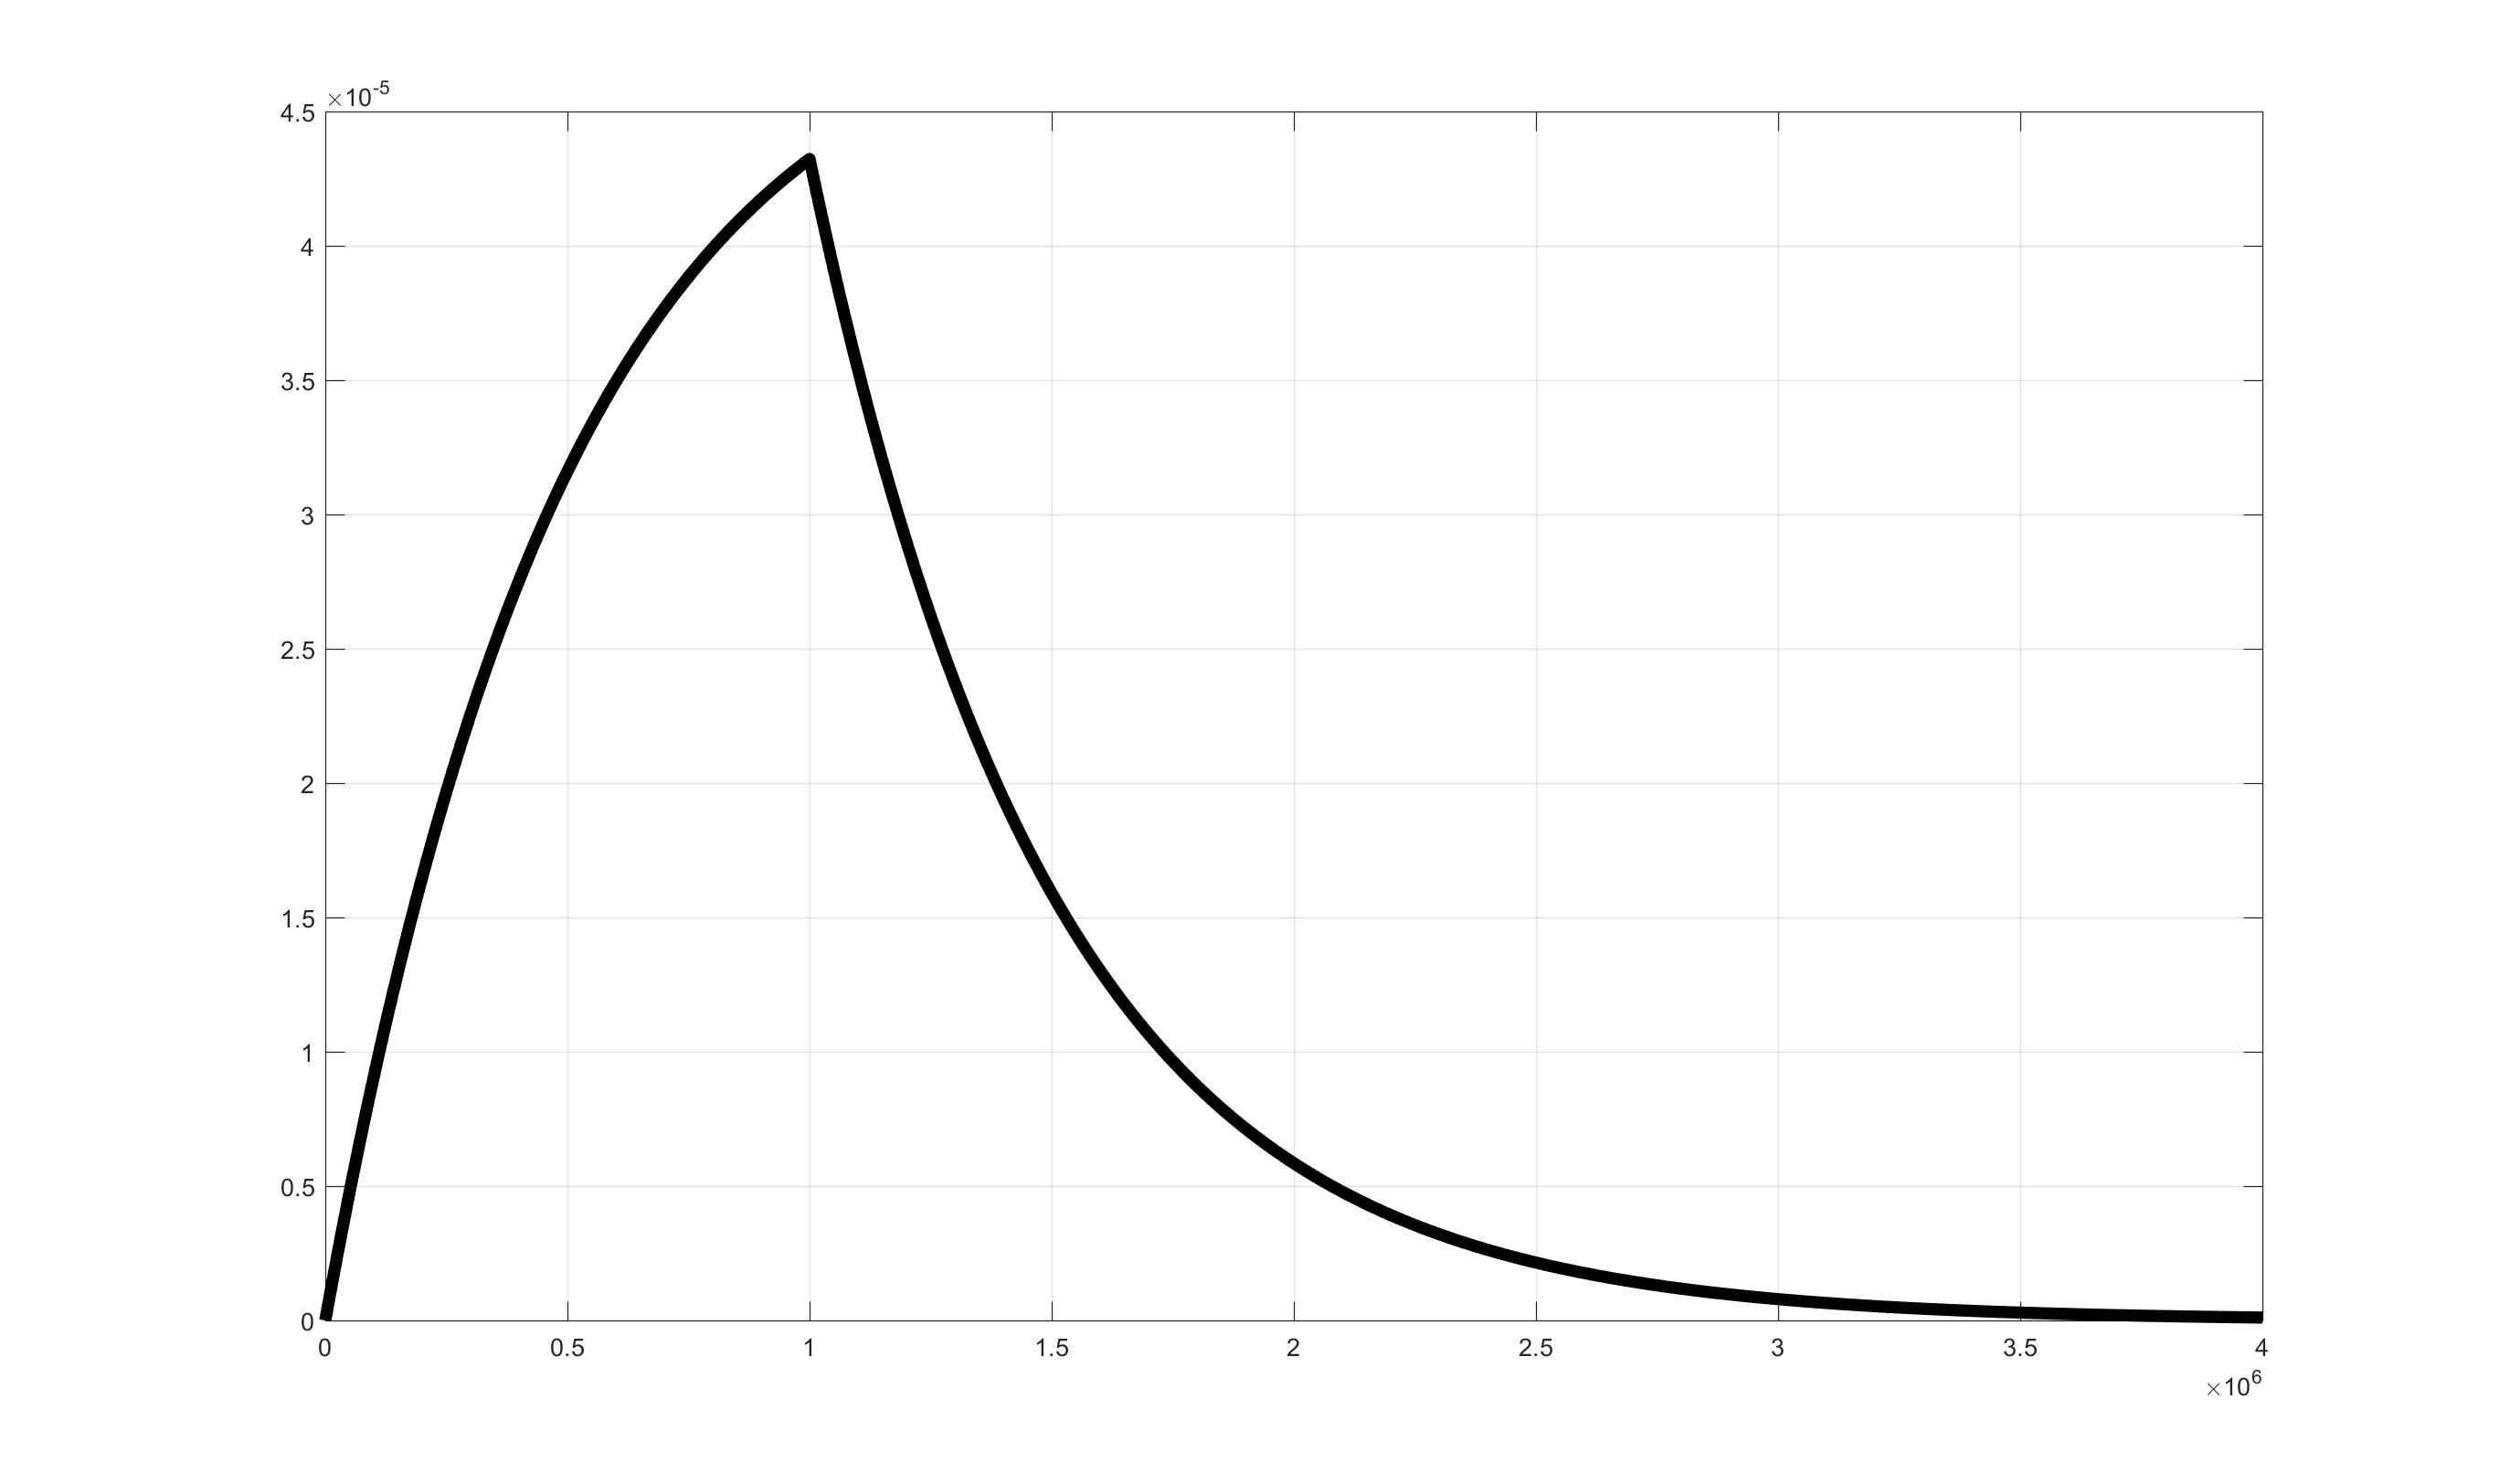
\includegraphics[width=0.9\textwidth]{ass1.jpg} 
  \caption{The concentration of the pollutant.} 
  \label{img} 
\end{figure}


%----------Problem 4----------
\vspace{2em}
\par
\begin{Large}
\textit{Problem 4.}
\end{Large}
\vspace{0.5em}
\\
\textit{a)}\,\,\,\textit{1)} For $x\neq 0$, 
$$1-(\frac{y}{x})^2+2\frac{y}{x}y'=0$$
$$y'=\frac{(\frac{y}{x})^2-1}{2\frac{y}{x}}$$
Let $v=\frac{y}{x}$,
$$y'=f(v)=\frac{v^2-1}{2v}$$
$$f-v=-\frac{v}{2}-\frac{1}{2v}$$
$$as \frac{y}{x}\neq 0, v\neq 0$$
Therefore we get
$$\int\frac{dv}{-\frac{v}{2}-\frac{1}{2v}}=\int\frac{dx}{x}$$
$$\int -\frac{2v}{v^2+1}dv=\int-\frac{d(v^2)}{v^2+1}=-ln(v^2+1)=ln|x|+c_1$$
$$e^{-\frac{d(v^2)}{v^2+1}}=e^{ln|x|+c_1}$$
$$\frac{x^2}{y^2+x^2}=c_2x$$
$$y=\pm\sqrt{c_2x-x^2}\,,\,c_2=const$$
Note that for $x=0$, we get $y=0$, and the solution above is also satisfied.\\
\\
\textit{2)}\,\,Use the properties of the exact equations, we get
$$P(x,y)=ln(y^2+1)\,,\,Q(x,y)=\frac{2y(x-1)}{y^2+1}$$
From the original equation, when $x=1$, $ln(y^2+1)=0$, thus $y=0$.
There exists a function $f(x,y)$ where 
$$f_x(x,y)=P(x,y),f_y(x,y)=Q(x,y)$$
Then
$$f(x,y)=\int f_x(x,y)dx=\int  ln(y^2+1)dx$$
$$=xln(y^2+1)+g(y)$$
where $g(y)$ is is an arbitrary function of $y$.
As $f_y(x,y)=Q_x$
$$\frac{2yx}{y^2+1}+g'(y)=\frac{2yx}{y^2+1}-\frac{1}{y^2+1}$$
$$g(y)=\int-\frac{1}{y^2+1}dy=-arctan(y)+c_1$$
The general solution has the form:
$$xln(y^2+1)-arctan(y)=c_2=0$$
The solution of the ODE is:
$$xln(y^2+1)-arctan(y)=0.$$
\\
\textit{3)}\,\,The original equation is a Bernoulli Equation, then divide both sides by $y^5$, get
$$\frac{y'}{y^5}+(-\frac{1}{2x})y=10x^2=-\frac{1}{4}(y^{-4})'+(-\frac{1}{2x})y=10x^2$$
Let $z=y^{-4}$,
$$z'+\frac{2}{x}z=-40x^2$$
$$Let\; \mu=e^{\int\frac{2}{x}dx}=c_2e^{x^2}$$
Thus,
$$z=\frac{1}{c_2x}(\int C_2x^2(-40)x^2dx+c_3)$$
$$=\frac{-8x^5}{x^2}+\frac{c_4}{x^2}$$
The solution for the ODE is
$$y^{-4}=-8x^3+\frac{c_4}{x^2}$$
\\
\textit{4)}\,\,For $x\neq 0$, the original equation can be expressed as:
$$y'=\frac{x-1}{2x^2}y^2+\frac{y}{x}+\frac{1-x}{2}$$
Guess a particular solution: $y_1=x$, then make the substitution:$y=y_1+\frac{1}{w}$, we get the linear equation:
$$w'+(\frac{1}{x}+\frac{x-1}{x})w=\frac{1-x}{2x^2}$$
The solution for $w$ is given:
$$w=\frac{1}{c_1e^x}(\int c_1e^x\frac{1-x}{2x^2}dx+c-2)$$
$$=\frac{1}{c_1e^x}(-c_1\frac{e^x}{2x}+c_3)$$
$$=\frac{-e^x+c_4x}{2x\cdot e^x}$$
Thus,
$$y=y_1+\frac{1}{w}=\frac{c_4x^2+xe^x}{c_4x-e^x}$$
where $c_4$ is a constant, depending on the initial condition.
\vspace{2em}
\\
\textit{b)}\,\,By using a suitable integrating factor, we can convert a differential equation that is not exact into an exact differential equation by multiplication.\footnote{This part of interpretation is cited from 'Elementary Differential Equations and Boundary Value Problems', 11th edition, pp.73-74. Willam E. Boyce, et.al.} For example, consider an equation 
\begin{equation}
M(x,y)+N(x,y)y'=0 
\end{equation}
%23
chooose a function $\mu$ and multiply it with the equation above so that
\begin{equation}
\mu(x,y)M(x,y)+\mu(x,y)N(x,y)y'=0
\end{equation}
%24
is exact, which indicates:
\begin{equation}
(\mu M)_y=(\mu N)_x
\end{equation}
Since M and N are given functions, equation (1) states that the integrating factor $\mu$ must satisfy the first-order partial differential equation
\begin{equation}
M\mu_y-N\mu_x+(M_y-N_x)\mu =0
\end{equation}
If a function $\mu$ satisfying equation (4) can be found, then equation (2) will be exact. The solution of equation (2) can then be obtained by the method described in the first part of this section. The solution found in this way also satisfies equation (1), since the integrating factor $\mu$ can be cancelled out of equation (2).\\
\\
\textit{c)}\,\,When $x\neq 0$, use the method of integrating factors:
$$y'-\frac{1}{x}y=0$$
define $\mu=c_1\cdot e^{\int(-\frac{1}{x})dx}=c_1e^{-ln|x|}=\frac{c_2}{x},$
then 
$$y=\frac{1}{\mu(x)}(\int(-\frac{1}{x})\cdot 0dx+c_3)=c_4\cdot x$$
where $c_4=const.$\\

When $x=0$, $y=0$, the situation is also satisfied.




\end{document}